\section*{Introducción al Código SQUAWK}
En la aviación, los transpondedores y los códigos Squawk son utilizados para minimizar las comunicaciones por voz, debido a la saturación de las frecuencias aeronáuticas. El Squawking es, en esencia, una forma de comunicación aire-tierra (controladores-pilotos) esencial para la seguridad y para tener un control de tráfico fluido y eficaz.

El código Squawk no es más que un código octal de 4 dígitos (4096 combinaciones únicas) que identifica la aeronave. 

La aeronave recibe una señal de interrogación por parte del SSR a 1030 MHz, a la que el transpondedor responde en una frecuencia de 1090 MHz. El transpondedor, aparte del código Squawk (modo $A$), puede incluir más información si está en modo $C$ (altitud) o modo $S$.

El controlador encargado de las autorizaciones (<<\textit{clearance delivery}>>) proporciona un Squawk a los pilotos, que identificará al vuelo. Asimismo, también existen varios códigos reservados, como el 7000 (VFR), el 7500 (secuestro), el 7600 (pérdida de radio) o el 7700 (emergencia), entre otros.

La codificación, en pulsos digitales (valor 0 ó 1) es como sigue:
\begin{equation*}
    F_1 \; C_1 A_1 C_2 A_2C_4 A_4 \; X \; B_1D_1B_2D_2B_4D_4
\end{equation*}

Siendo $F_1$ y $F_2$ los pulsos que marcan el inicio y el final de la secuencia respectivamente, $X$ siempre toma el valor 0, y los dígitos $A_i, \, B_i,\, C_i, D_i$ son la codificación binaria (con el código Squawk siendo ABCD). De tal manera que, por ejemplo, el Squawk 1234 se codificaría como:

\begin{equation*}
    \underbrace{1}_{F_1} \; \overbrace{ 1 1 1 0 0}^{C_i \; A_i} \; \underbrace{0}_X\; \overbrace{0 0 1 0 1 0}^{B_i \; D_i} \; \underbrace{1}_{F_2}
\end{equation*}


\section*{Circuito}
El circuito (\cref{fig:circuito}) se compone de:
\begin{itemize}
    \item \textbf{Doce microinterruptores} (como los de la \cref{Microinterruptores}), etiquetados como \texttt{DSW1} en el circuito, que corresponden a las variables anteriormente descritas ($C_i, \, A_i, \, B_i,\, D_i$). 
    \item \textbf{Dos  barras de resistencias} (como las de la \cref{Resistencias}), etiquetadas como \texttt{BARRA 1} y \texttt{BARRA 2} en el circuito.
    \item \textbf{Oscilador de 1 MHz} (\cref{Oscilador}), etiquetado como \texttt{OSCILADOR} en el circuito. Genera la señal de reloj necesaria.
    \item \textbf{GAL G22V10} (\cref{GAL}), etiquetada como \texttt{GAL} en el circuito. Es el <<\textit{cerebro}>> del circuito que programamos con el código descrito en las siguientes páginas.
\end{itemize}


\begin{figure}[!htb]
    \centering
    
    \begin{minipage}{.4\textwidth}
        \centering
        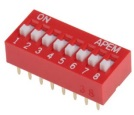
\includegraphics[width=0.6\linewidth]{include/figures/Microinterruptores.jpg}
        \captionof{figure}{Microinterruptores}
        \label{Microinterruptores} 
    \end{minipage}
    \begin{minipage}{.4\textwidth}
        \centering
        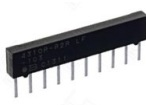
\includegraphics[width=0.5\linewidth]{include/figures/Barra.jpg}
        \captionof{figure}{Barra}
        \label{Resistencias} 
    \end{minipage}
    
    \begin{minipage}{.4\textwidth}
        \centering
        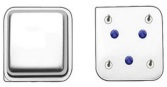
\includegraphics[width=0.6\linewidth]{include/figures/Oscilador.jpg}
        \captionof{figure}{Oscilador}
        \label{Oscilador} 
    \end{minipage}
    \begin{minipage}{.4\textwidth}
        \centering
        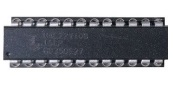
\includegraphics[width=0.5\linewidth]{include/figures/GALg22v10.jpg}
        \captionof{figure}{GAL G22V10}
        \label{GAL} 
    \end{minipage}

\end{figure}

\begin{figure}[!htb]
    \centering
    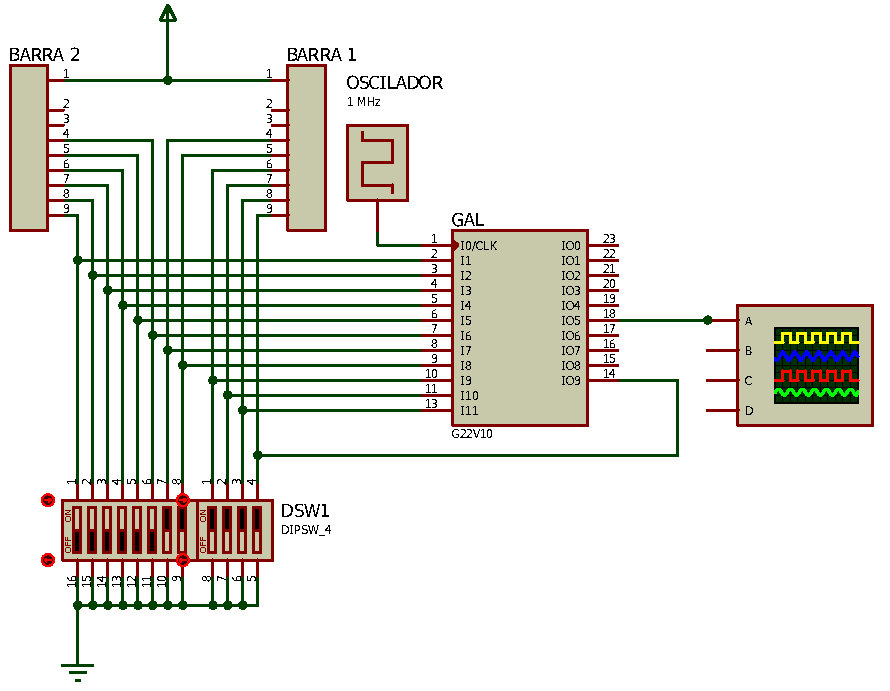
\includegraphics[width=\linewidth]{include/figures/esquema.pdf}
    \caption{Captura del circuito en <<\textit{Proteus}>>}
    \label{circuito-proteus}
\end{figure}

% Como include para que no se corte
\section*{Ecuaciones}
El código está disponible en GitHub (\textcolor{blue}{\href{https://github.com/IvanMoyaO/SQUAWK-GAL}{https://github.com/IvanMoyaO/SQUAWK-GAL}}) y en las siguientes páginas. 

La estructura del código es la siguiente:
\begin{itemize}
    \item \textbf{Cabecera y declaración de entradas y salidas}: en las primeras 36 líneas, se establece la cabecera del programa (con información como la fecha o el dispositivo) y se declaran qué pines se usarán como entradas/salidas y qué variable tendrán asignada. Nótese que la variable los pulsos, $Z$, se asigna al pin 18 en concreto debido al número de términos que tiene.
    \item \textbf{Ecuaciones del contador}: entre las líneas 38 y 58 se realizan las ecuaciones de un contador sencillo, sin truncar y que cuenta todos lo números.
    \item \textbf{Variables intermedias}: entre las líneas 63 y 77 se declaran una serie de variables intermedias que corresponden a los instantes en los que habrá un pulso. Esta parte no es necesaria, sin embargo, consideramos que favorece enormemente la legibilidad.
    \item \textbf{Salida}: en la línea 79 se establece el valor (1 ó 0) de la salida. Solo se activará en determinados instantes si, y solo si, el correspondiente microinterruptor está activo.
\end{itemize}

\begin{cuidado}{Errores que cometimos}
En la primera versión del código, \textcolor{blue}{\href{https://github.com/IvanMoyaO/SQUAWK-GAL/commit/ac02036bc24f1b977cd46d78ace5171c46c0033c}{como puede verse en GitHub}}, los pulsos que generamos no se asemejaban a un código SQUAWK debido a que faltaba $X$, $F_1$ y $F_2$.

\textcolor{blue}{\href{https://github.com/IvanMoyaO/SQUAWK-GAL/commit/d1294f0a59ebac4c123ad7443a96185edbf2dbca}{Una versión posterior}} añadió dichos pulsos, pero seguía siendo incorrecta al no dejar un <<\textit{tiempo muerto}>> tras $F_2$. \textcolor{blue}{\href{https://github.com/IvanMoyaO/SQUAWK-GAL/commit/8cf73270ac348ffd79384d2d9c017e38601c2216}{Los cambios que introdujo definitiva pueden verse en GitHub}}.

\end{cuidado}

El código/ecuaciones se recoge a continuación:

\lstset{inputencoding=utf8/latin1}
\lstinputlisting[
frame=single,
numbers=left,
breaklines=true
]{ecuaciones.pld}



\section*{Realización del Circuito en el Laboratorio}
Una vez verificado el circuito y las ecuaciones por el profesor, procedimos al montaje del circuito en el laboratorio. 

En el laboratorio, nos guiamos del esquema obtenido de <<\textit{Proteus}>>, mostrado anteriormente en la \cref{circuito-proteus}, para la realización del circuito en una <<\textit{Protoboard}>> (\cref{Protoboard}).

    \begin{figure}[!htb]
        \centering
        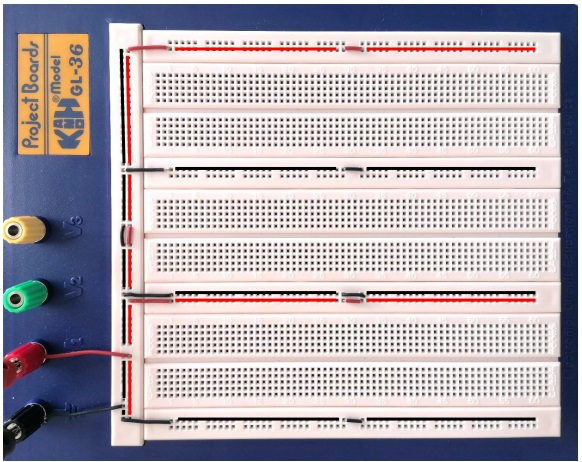
\includegraphics[width=0.5\linewidth]{include/figures/Protoboard.jpg}
        \caption{<<\textit{Protoboard}>>}
        \label{Protoboard}
    \end{figure}
    

Para la programación de la GAL se usó <<\textit{Xgpro}>> a través del programador \texttt{TL866-II}.

\begin{figure}[!htb]
    \centering
    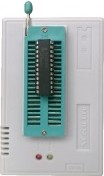
\includegraphics[width=0.14\linewidth]{include/figures/Programador.jpg}
    \caption{Programador TL866-II}
    \label{Programador}
\end{figure}

\begin{cuidado}{Problema que tuvimos}
A la hora de programar la GAL, <<\textit{Xgpro}>> arrojaba un error. A pesar de probar diversas soluciones, ninguna resultó. Sin embargo, a pesar de dar error, sí que se estaba programando la \texttt{GAL}. Posteriormente resultó que el error se debía a que había un carácter extraño en el fichero \texttt{.jed}, seguramente debido a que se había compilado en un entorno Linux ejecutando <<\textit{WINCUPL}>> a través de <<\textit{Wine}>>.
\end{cuidado}


Una vez completado el circuito, conectamos el oscilador y la fuente de alimentación. El circuito, una vez montado, se ilustra en la figura \ref{fig:circuito}.

\begin{figure}[!htb]
    \centering
    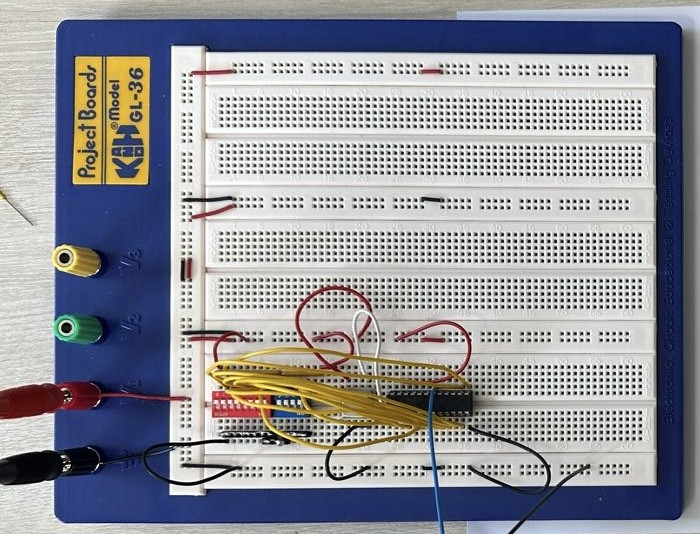
\includegraphics[width=0.45\linewidth]{include/figures/Circuito.jpg}
    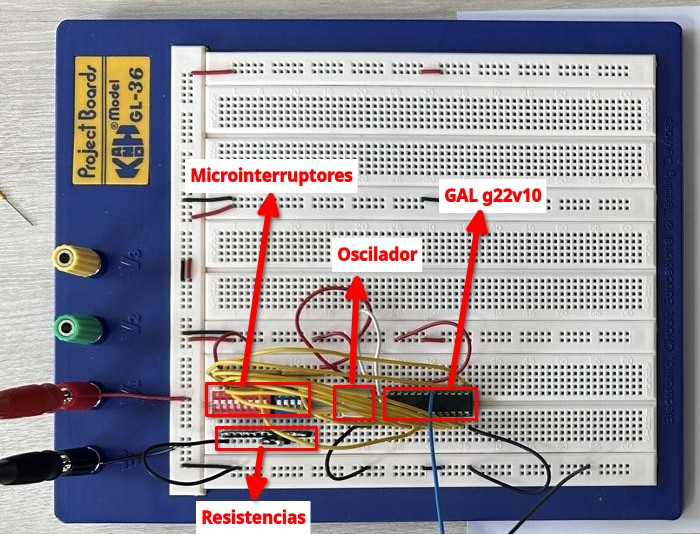
\includegraphics[width=0.45\linewidth]{include/figures/circuito-anotado.jpg}
    \caption{Circuito}
    \label{fig:circuito}
\end{figure}


En el osciloscopio, una vez ajustadas las franjas de tiempo, observamos, como esperábamos, pulsos de duración 1 $\mu s$ cada 2$\mu s$ (\cref{Osciloscopio}). Asimismo, comprobamos que, al variar la posición de los microinterruptores, desaparecían los pulsos correspondientes.

\begin{figure}[!htb]
    \centering
    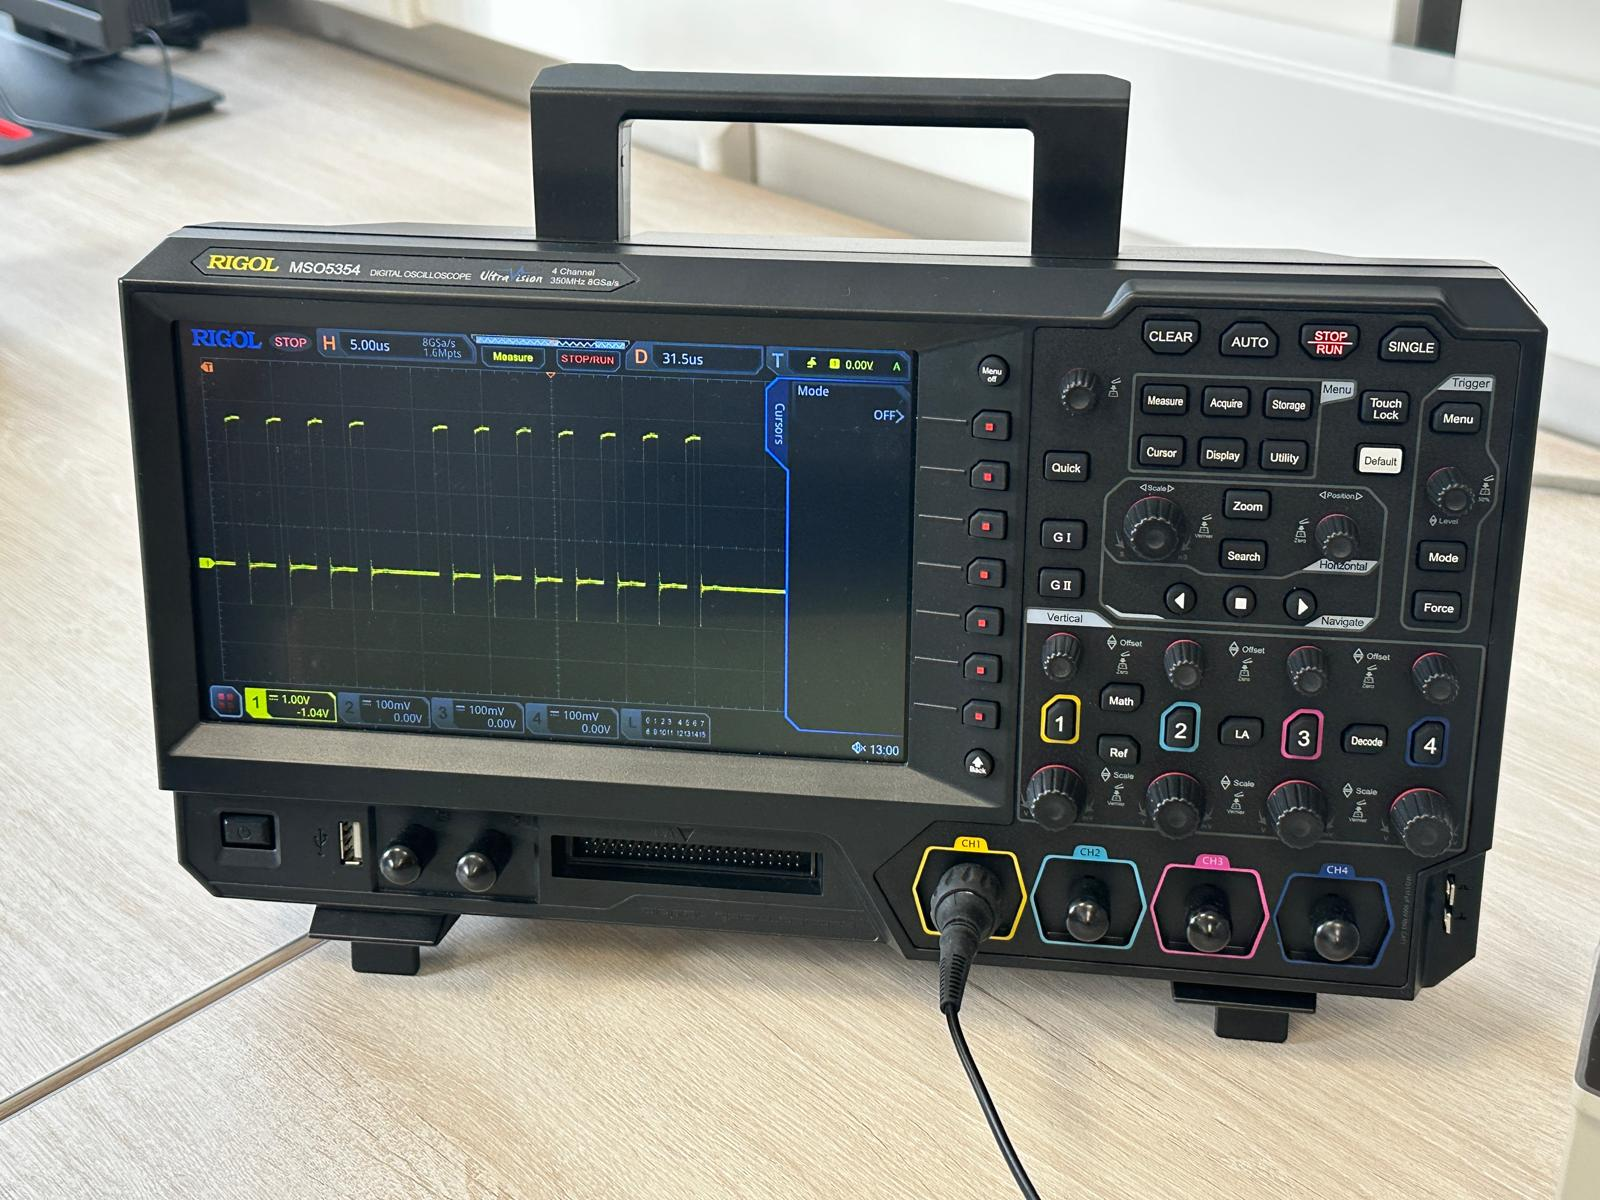
\includegraphics[width=0.5\linewidth]{include/figures/Osciloscopio.jpg}
    \caption{Osciloscopio}
    \label{Osciloscopio}
\end{figure}
